
\subsection{{Description}}

    {In Problem Set 3, ALU undergoes a significant modification in its Control Unit, specifically focusing on the Finite State Machine (FSM) sub-component. The task involves utilizing the studentId output from the FSM sub-component and integrating it into the ALU design, enabling the ALU to process four inputs, as detailed in this lab report.}

    \subsubsection{{Inputs}}

        \begin{itemize}
            \item   {\textbf{A (8-bit)}: First input of 8 bits for arithmetic and logical operations.}
            \item   {\textbf{B (8-bit)}: Second 8-bit input for arithmetic and logical operations.}
            \item   {\textbf{Control Unit (16-bit)}: Microcode input from the control unit, functioning as the operation-selector signal.}
        \end{itemize}

    \subsubsection{{Outputs}}

        \begin{itemize}
            \item   {\textbf{Result (8-bit)}: Output representing the result of operations performed on inputs A and B.}
            \item   {\textbf{7-Segment Displays/LEDs}: Display output in hexadecimal format during FPGA board implementation.}
        \end{itemize}

    \subsubsection{{Purpose}}

        \begin{itemize}
            \item   {\textbf{A and B}: Serve as inputs for arithmetic and logical operations.}
            \item   {\textbf{Control Unit}: Determines the operation to be applied to inputs A and B.}
            \item   {\textbf{Result}: Represents the output of operations on A and B.}
            \item   {\textbf{7-Segment Displays/LEDs}: Display the output in hexadecimal format during FPGA board implementation.}
        \end{itemize}
    
    \subsubitem{{Design}}

        {ALU's design integrates the modified FSM sub-component into the Control Unit, incorporating the studentId output. The specific modification involves assessing whether one of the two digits of input A is less than the FSM output (studentId), assigning 'Y' if true and 'N' otherwise (Problem 3 Part C). This modification aligns with the lab's overarching objectives, leveraging microcode instructions from the initial design section.}

        {The implementation process includes synthesizing and simulating ALU's functionality. The modified ALU is then verified, and results, including waveforms and potential adjustments to 7-segment displays for 'Y' or 'N' visualization, are presented in the final report submission. ALU's role is critical in adapting the control unit to process additional inputs, enhancing the versatility and applicability of the ALU within the GPU unit.}
    
    \subsubsection{{Timing Diagram}}

    \begin{figure}[H]
        \centering
        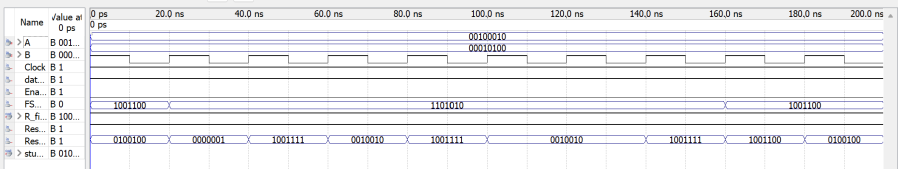
\includegraphics[width=15cm]{Pictures/ALU3WaveForm.png}
        \caption{{Timing Diagram of the Complete Logic Circuit 3}}
        \label{}
    \end{figure}

    \subsubsection{{Block Diagram}}

        \begin{figure}[H]
            \centering
            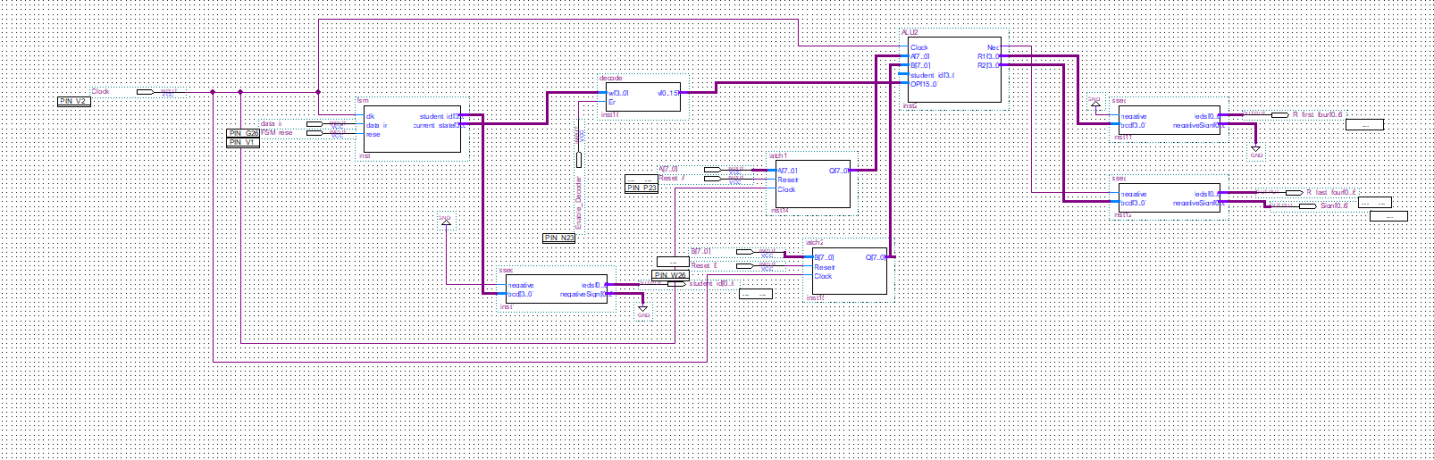
\includegraphics[width=15cm]{Pictures/P12BlockDia.png}
            \caption{{Block Diagram of the Complete Logic Circuit 3}}
            \label{}
        \end{figure}

%\subsection{{VHDL Code}}

%    \subimport{./}{P3-VHDL}

